% Study of measurement, objectives, and search strategies for tuning OpenMP
% offload kernels with kernel record and replay.
% References are in references.bib; figures are generated by figures/make_figures.py.
\documentclass[10pt]{article}
\usepackage[margin=1in]{geometry}
\usepackage[T1]{fontenc}
\usepackage{lmodern}
\usepackage{amsmath,amssymb}
\usepackage{booktabs}
\usepackage{multirow}
\usepackage{array}
\usepackage{xcolor}
\usepackage{graphicx}
\graphicspath{{figures/}}
\usepackage[hidelinks]{hyperref}

\newcommand{\x}{\ensuremath{\times}}
\newcommand{\code}[1]{\texttt{#1}}
\newcommand{\pending}[1]{\textcolor{red}{#1}}

\title{Measurement, Objectives, and Search Strategies for Tuning OpenMP Offload Kernels with Kernel Record and Replay}
\author{Technical report, \code{openmp-rr} repository, branch \code{measurement-v3}}
\date{October 2026}

\begin{document}
% Long monospace identifiers cannot be hyphenated; allow looser spacing instead
% of overfull lines.
\sloppy
\maketitle

\begin{abstract}
Kernel record and replay lets an autotuner evaluate one GPU kernel of an
OpenMP offload application in isolation, so that each tuning experiment costs
a single kernel launch instead of a full application run. The existing tuner
in this repository uses Bayesian optimization over four launch parameters and
can target speedup, energy, or global memory loads and stores. We set out to
answer two questions: whether knowledge of all of these metrics leads to
better kernel configurations, and whether a technique better than Bayesian
optimization exists. We find that measurement, rather than the search
algorithm, limited the existing results. Replay timings were taken while the
GPU clock was still ramping up from idle, so the same configuration varied
by 8.4\% between processes and the reported best speedups of most kernels
did not replicate. Energy was measured around the whole replay process, and
the load and store counters count instructions, which do not change with the
launch configuration. After we fixed the measurement, cross-process variation
fell to 0.23\%. With clean measurements, Bayesian optimization, the
tree-structured Parzen estimator (TPE), and multi-objective TPE ship equally
fast configurations on ten LULESH kernels, while random search is 5\% slower.
Knowledge of energy does not find faster configurations, but time-optimal and
energy-optimal configurations always differ, by up to 1.83\x{} in energy on
one kernel. Metrics that do vary with the launch configuration (DRAM traffic,
cache hit rate, register spills, occupancy, and SM pipe utilization) explain
the large gains and predict when a kernel has nothing to gain. A pipeline that
classifies each kernel's bottleneck from baseline metrics and chooses the
search strategy accordingly matches or beats every fixed strategy, measures
30\% fewer configurations on LULESH, and improves on Bayesian optimization by
1.3\% on held-out miniFE kernels. Finally, we test four avenues for searching
faster online. Multi-fidelity screening, a warm start from other kernels'
best configurations, a cost model transferred across kernels, and a
prior-guided acquisition each reach good configurations much earlier, for
example 0.74 instead of 0.42 of the attainable gain within the cost of ten
full evaluations, and ship 1.0\% to 1.9\% faster configurations. Replaying many
configurations in one process, with the inputs restored on the device between
them, cuts the cost of a configuration from about 4~s to 0.5~s, and with the
same 300~s budget it ships 6.8\% faster configurations than screening with
one process per configuration. Adding a convergence-based stop to batch
screening gives the same quality in about half the time, roughly 2.5 minutes
per kernel instead of about 15 for Bayesian optimization with 60 full
evaluations.
\end{abstract}

\tableofcontents

%=============================================================================
\section{Introduction}
\label{sec:intro}

Choosing the launch configuration of a GPU kernel is a classic autotuning
problem. For an OpenMP offload kernel, the configuration consists of the
number of \emph{teams} (CUDA thread blocks), the number of threads per team,
and compiler hints that bound the block size and the number of resident
blocks. The best values depend on the kernel, the input, and the GPU, and a
poor choice can make a kernel several times slower than necessary.
Parasyris et al.\ showed that kernel record and replay makes such tuning
practical for whole applications, because a recorded kernel can be replayed
in isolation with any configuration, and they reported a 1.53\x{} end-to-end
speedup on LULESH with tuning 102\x{} faster than tuning the whole
application~\cite{parasyris2023rr}.

The tuner in this repository builds on that work. It searches four launch
parameters with Bayesian optimization (BO) and can optimize speedup, energy,
global load requests, global store requests, or their product. We were asked
whether knowledge of all of these metrics leads to better configurations,
and whether a better search technique than BO exists. Answering either
question requires measurements that are accurate enough to compare
configurations, so the study grew into an examination of the measurement
pipeline itself.

In this work, we make the following contributions:
\begin{itemize}
\item We show that the existing measurements could not support the existing
  conclusions. Timing varied by 8.4\% across replay processes because of the
  GPU clock ramp, reported winners lost most of their speedup when
  re-measured, energy was process energy, and the load and store counters
  are invariant to the launch configuration (Section~\ref{sec:offline}).
\item We fix the measurement with a time-based warm-up, repeated
  event-timed launches, kernel-level energy, a GPU exclusivity guard, and
  warmed-up profiling, and we reduce cross-process variation from 8.4\% to
  0.23\% (Sections~\ref{sec:measurement} and~\ref{sec:adaptive}).
\item We compare five search strategies online on ten LULESH kernels with
  ground-truth validation, and find that model-based strategies tie while
  random search is significantly worse (Section~\ref{sec:search}).
\item We show that energy-aware and multi-objective search find the
  time-energy trade-off at no cost in speed, and we identify which hardware
  metrics vary with the launch configuration and explain performance
  (Sections~\ref{sec:search} and~\ref{sec:metrics}).
\item We propose and evaluate a bottleneck-adaptive tuning pipeline, test it
  on held-out miniFE kernels, and quantify further avenues for reaching good
  configurations with fewer evaluations
  (Sections~\ref{sec:targets} to~\ref{sec:efficiency}).
\end{itemize}

%=============================================================================
\section{Background and terminology}
\label{sec:background}

This section defines the terms used in the rest of the report.

\subsection{OpenMP offload and launch parameters}
An \emph{OpenMP offload kernel} is a loop region annotated with
\code{\#pragma omp target teams distribute parallel for}. The LLVM OpenMP
runtime (\code{libomptarget}) launches it on the GPU as a CUDA kernel. A
\emph{team} corresponds to a CUDA thread block, and the threads of a team
execute loop iterations. If there are fewer threads in total than loop
iterations, each thread executes several iterations in a \emph{grid-stride}
loop. The \emph{trip count} is the number of loop iterations.

The tuner controls four parameters. \code{NumThreads} is the number of
threads per team, and \code{NumTeams} is the number of teams. Both are runtime
parameters, so changing them needs no recompilation. \code{MaxThreads} and
\code{MinTeams} are \emph{launch bounds}, hints passed to the NVPTX backend
by an LLVM pass in this repository. They correspond to the CUDA
\code{\_\_launch\_bounds\_\_} attributes \emph{maxThreadsPerBlock} and
\emph{minBlocksPerMultiprocessor}. They tell the register allocator how many
threads must fit on a streaming multiprocessor (SM), so they change the
number of registers per thread, and they can force \emph{register spills},
which move values that do not fit in registers to \emph{local memory} (a
per-thread region of device memory). Changing a launch bound requires
recompiling the kernel image.

The tuner searches a normalized space in which each parameter is a fraction
in $(0, 1]$. A fraction is mapped to a discrete configuration as follows.
\code{MaxThreads} is the fraction of 32 warps per block, rounded up to a
multiple of the warp size of 32 threads. \code{MinTeams} is the fraction of
the largest number of blocks of that size that fit on one SM (at most 32).
\code{NumThreads} is the fraction of \code{MaxThreads}, rounded to a warp
multiple. \code{NumTeams} is the fraction of the number of teams that would
give each thread exactly one iteration, that is,
$\lceil \text{trip count} / \text{NumThreads} \rceil$. We call the product
$\text{NumTeams} \times \text{NumThreads} / \text{trip count}$ the
\emph{teams fraction}. A teams fraction of 1 means one iteration per thread,
and a smaller value means a grid-stride loop. The \emph{baseline} is the
configuration that the compiler and runtime choose without tuning.

\subsection{GPU performance concepts}
\emph{Occupancy} is the ratio of active warps on an SM to the maximum the SM
supports. \emph{Theoretical occupancy} follows from the block size, the
registers per thread, and shared memory use, and \emph{achieved occupancy}
is measured during execution. A \emph{wave} is one round of thread blocks
that fills every SM, so the number of waves is the number of teams divided
by the number of SMs times the blocks that fit per SM. When the last wave is
only partly full, the GPU is underused at the end of the kernel, which we
call the \emph{tail effect}. A kernel is \emph{memory bound} when DRAM
bandwidth limits it and \emph{compute bound} when its arithmetic pipelines
do. We use \emph{locality bound} for a memory-bound kernel whose DRAM traffic
can be reduced by better cache reuse, and \emph{register bound} for a kernel
whose performance is limited by register pressure, through low occupancy or
spills. The NVIDIA T4 used here executes double-precision (FP64) arithmetic
at 1/32 of its single-precision rate, so FP64-heavy kernels saturate the FP64
pipe early.

\subsection{Measurement tools}
\emph{CUDA events} time a kernel on the GPU. \emph{NVML} (NVIDIA Management
Library) reports the board's cumulative energy counter and clock speeds.
\emph{CUPTI} (CUDA Profiling Tools Interface) and its \emph{perfworks}
metrics API collect hardware counters. A metric such as
\code{dram\_\_sectors\_read.sum} counts 32-byte sectors read from DRAM, and a
metric such as \code{sm\_\_throughput.avg.pct\_of\_peak\_sustained\_elapsed}
reports utilization as a percentage of the peak rate. Collecting many
counters needs several passes, so CUPTI \emph{kernel replay} re-runs the
kernel once per pass and restores its memory between passes. The repository
wraps this API in a small library called \code{nvmetrics}.

\subsection{Kernel record and replay}
During a \emph{recording}, the runtime saves each kernel's device memory, its
arguments, its global variables, and its device image. During a
\emph{replay}, the tool \code{llvm-omp-kernel-replay} loads one recorded
kernel into a fresh process, launches it with a chosen configuration, and can
compare the output against the recorded output. Each replay is a separate
operating system process, so every measurement pays for process start-up and
for loading the recorded memory (2 GB for LULESH, about 3 GB for miniFE).

\subsection{Search strategies}
\emph{Bayesian optimization} (BO) fits a probabilistic surrogate model to the
configurations measured so far and chooses the next configuration by
maximizing an \emph{acquisition function}. The existing tuner uses the
\code{bayes\_opt} library~\cite{nogueira2014bayesopt}, a Gaussian process
(GP) surrogate with a Mat\'ern kernel, and the upper confidence bound (UCB)
acquisition~\cite{srinivas2010gpucb} with $\kappa = 1.96$. \emph{Expected
improvement} (EI) is the expected amount by which a candidate exceeds the
best value found so far~\cite{jones1998ego}. The \emph{tree-structured Parzen
estimator} (TPE) models the density of good and bad configurations separately
and proposes points where their ratio is high~\cite{bergstra2011tpe}. We use
the Optuna implementation~\cite{akiba2019optuna}, including its
multi-objective variant (MOTPE)~\cite{ozaki2022motpe}. \emph{ExtraTrees}
(extremely randomized trees) is a tree ensemble regressor~\cite{geurts2006extratrees}.
We use it as a surrogate whose per-tree spread provides the uncertainty for
EI, as in SMAC-style optimizers. \emph{Random search} samples configurations
uniformly. An \emph{initial design} is the set of configurations evaluated
before the surrogate is first used, and a \emph{budget} is the number of
configurations a search may propose.

\subsection{Statistics}
The \emph{coefficient of variation} (CV) is the standard deviation divided by
the mean. We report speedups as ratios and average them with the geometric
mean. The \emph{share of attainable gain} of a result is
$\log(\text{speedup}) / \log(\text{best known speedup})$, so 1 means the best
configuration known for the kernel. \emph{Spearman's} $\rho$ and
\emph{Kendall's} $\tau$ are rank correlations. A \emph{Pareto front} is the
set of configurations that no other configuration beats in both time and
energy, and the \emph{hypervolume} is the area that the front dominates
relative to a reference point (here the baseline), so a larger hypervolume
means a better set of trade-offs. A \emph{kernel-clustered bootstrap}
resamples kernels with replacement, which gives a confidence interval (CI)
that accounts for the correlation of results within a kernel. The
\emph{winner's curse} is the upward bias in the best of many noisy
measurements, so a reported best value tends to shrink when re-measured.

%=============================================================================
\section{Experimental setup}
\label{sec:setup}

\textbf{Hardware and software.} All experiments ran on one node with eight
NVIDIA Tesla T4 GPUs (Turing, compute capability 7.5, 40 SMs, 16 GB, 70 W
board power limit), NVIDIA driver 610.57.04. Builds and runs used the
Apptainer container \code{rr\_current.sif} with GCC~12 and the LLVM~16-based
OpenMP runtime in this repository (nextgen CUDA plugin). Jobs ran inside named
\code{tmux} sessions, with logs and exit codes kept in
\code{experiment-archives/}.

\textbf{Applications.} We use LULESH, a shock hydrodynamics proxy
application~\cite{karlin2013lulesh}, recorded at commit \code{fdec6e319},
which has 17 recorded kernels, and miniFE, a finite element proxy
application~\cite{heroux2009mantevo}, with a $200^3$ problem and 7 recorded
kernels. We refer to a kernel by the source line of its offload region, for
example l649. The online studies use ten LULESH kernels (333, 584, 649, 844,
1029, 1080, 1201, 1721, 1913, 2103) and all seven miniFE kernels (157, 169,
205, 210, 254, 290, 521).

\textbf{Search scenario.} All searches use the \code{BOMN} scenario of the
tuner, which searches all four parameters. Unless stated otherwise, a run
proposes 60 configurations, the model-based strategies start with 15
initial samples, and each strategy runs with three random seeds. The
existing workflow used 30 initial samples and 200 proposals.

\textbf{Ground truth.} Each search ships the configuration with the best
measured value of its objective. To compare strategies without the bias of
their own measurements, we re-measured every shipped configuration together
with the baseline in five rounds with randomized order, and we report the
median ratio within rounds as the \emph{true speedup}. The median standard
deviation of the log speedup across rounds was 0.003 to 0.004.

%=============================================================================
\section{Analysis of the existing optimizer results}
\label{sec:offline}

We first analyzed the databases that the existing tuner had produced, without
running new experiments. The comparable data were a LULESH run in which
independent speedup-objective and energy-objective BO searches each evaluated
230 configurations of 17 kernels, and miniFE speedup searches of seven
kernels. All used the same measurement method (schema
\code{device-kernel-timing-v2}): the duration of one event-timed launch per
replay process, five processes per configuration, and NVML energy measured
around each process.

\subsection{Measurement noise and the winner's curse}
Noise was large relative to the reported gains. Within one configuration, the
CV of the five replays had a median of 4.3\% and a 90th percentile of
12.6\%. We found 1779 configurations that both LULESH searches had measured.
The absolute log ratio of their two durations had a median of 0.072 and a
90th percentile of 0.231, which corresponds to 26\% disagreement at the 90th
percentile. The baseline alone differed by up to 32\% between the two
searches (l1913).

As a result, reported winners did not replicate. We took the five best
configurations of each search and looked them up in the other search. Their
median claimed speedup was 1.109\x{}, and their median speedup in the other
search was 1.003\x{}, a geometric shrinkage to 0.908 of the claim. For
example, l1913 fell from 1.47\x{} to 1.02\x{}, and l1721 fell from 1.23\x{}
to 0.85\x{} (Figure~\ref{fig:winners}). Only large effects survived, namely
l649 and l1029 at about 2.1\x{} to 2.2\x{}. The search trajectories tell the same story. The 30
random initial samples reached a median 83\% of the final log gain, and the
best configuration was found at a median of evaluation 145, usually as a 1\%
to 3\% improvement, which is within the noise.


\begin{figure}[t]
\centering
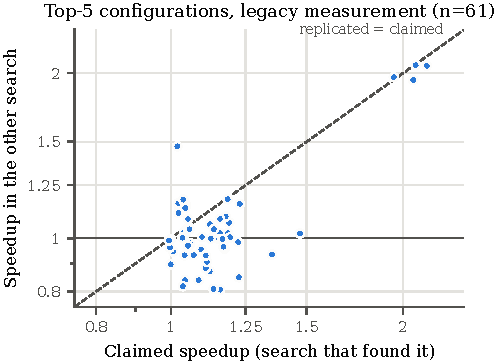
\includegraphics[width=0.48\textwidth]{winners_curse}
\caption{Winner's curse under the legacy measurement. Each point is one of the five best configurations of a LULESH search (x axis) looked up in the independent search of the same kernel (y axis). Points below the diagonal lost speedup when re-measured, and only the configurations near 2\x{} (l649 and l1029) replicated.}
\label{fig:winners}
\end{figure}
\subsection{Energy and memory metrics}
The energy objective measured process energy, not kernel energy. NVML
reported a median 86.4~J per replay process, while a 3.7~ms kernel at the
70~W limit can use at most 0.26~J. Across configurations, energy varied by
only 5\% to 6\% and had no rank correlation with duration (median Spearman
$\rho$ of 0.06 and $-0.03$ in the two searches). In the energy search, the
baseline was measured first, and its first replay drew 4.45\x{} the median
energy of its later replays, because the GPU and the file cache were cold.
This outlier inflated the baseline mean and produced the uniform 1.9\x{}
"energy gain" that the earlier report showed for every kernel. The
configuration that the energy search would ship ran at 0.98\x{} the baseline
speed on average.

The global load and store request counters did not vary with the launch
configuration on 16 of 17 LULESH kernels. These counters
(\code{l1tex\_\_t\_requests\_pipe\_lsu\_mem\_global\_op\_ld.sum} and its store
counterpart) count warp-level memory instructions. Every loop iteration
executes the same body regardless of how iterations are distributed, so the
instruction count is fixed by the code and the trip count. For example, the
store count of several kernels equals the number of mesh nodes divided by
32. The only kernels whose counts varied were reductions, because the OpenMP
runtime stores one partial result per team (Section~\ref{sec:metrics}).
Objectives built on these counters therefore gave the search no signal.

\subsection{Predictive value of the metrics}
We trained ExtraTrees models to predict the log duration and measured the
cross-validated Spearman correlation between predictions and measurements.
Launch parameters alone gave a median of 0.54 on LULESH and 0.71 on miniFE.
Adding compile-time registers, spills, and theoretical occupancy gave 0.58
and 0.69, and adding measured occupancy, loads, stores, and branch efficiency
gave 0.61 and 0.77. Within the best 10\% of configurations, no feature set
ranked configurations well (Spearman $\rho$ at most 0.12), because noise
dominated the differences there.

\subsection{Offline comparison of search strategies}
We built a benchmark from the 229 to 430 distinct configurations measured per
kernel. Each simulated evaluation returned the pooled measurement plus noise
resampled from the cross-run residuals, and each strategy was scored on the
true value of the configuration it would ship. Without noise, TPE reached
0.91 of the attainable gain after 60 evaluations, compared with 0.84 for the
existing GP-UCB, which was no better than random search before about 120
evaluations. With realistic noise, no strategy beat GP-UCB by a resolvable
margin, and searching longer made results worse, because more evaluations
gave more chances to ship a lucky outlier. Spending the last 15\% of the
budget on re-measuring the five best candidates improved the share of
attainable gain by 0.10 to 0.16 regardless of the strategy. This benchmark
contained only configurations that BO had chosen, which favors BO-like
strategies, and the online study in Section~\ref{sec:search} revises its
conclusion about random search.

We also found that 1810 of the evaluations in the miniFE databases repeated
a configuration already evaluated. The BO library proposes continuous points,
several of which round to the same discrete configuration, and a rerun with
the fixed random seed 1234 proposed the same points again.

%=============================================================================
\section{Fixing the measurement}
\label{sec:measurement}

\subsection{Root causes}
The dominant source of noise was the GPU clock ramp. A T4 at idle runs its SM
clock at about 600~MHz and raises it in steps to 1590~MHz over roughly
0.5~s of sustained load. A replay process launched its kernel within
milliseconds of starting, so each legacy sample was taken at a random point
of the ramp. Within one process, successive launches of l1721 stepped
through plateaus of 18.6, 16.8, 15.4, 12.7, 10.0, and 8.7~ms. After about
0.5~s of warm-up, the same kernel took 6.85~ms $\pm$ 0.3\% in every
process (Figure~\ref{fig:ramp}). A sweep of warm-up times showed that 500~ms sufficed for both a
long kernel (l1721) and a short one (l2103), and that warm-ups of 4~s began to
show small clock reductions from the power limit.


\begin{figure}[t]
\centering
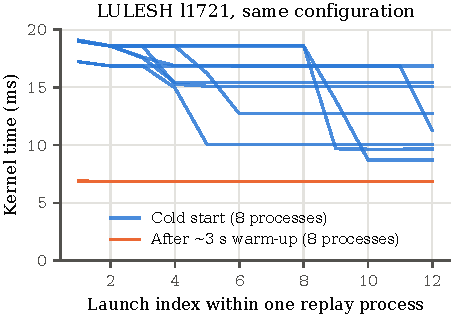
\includegraphics[width=0.48\textwidth]{clock_ramp}
\caption{Per-launch kernel time of the same LULESH l1721 configuration in eight replay processes started from an idle GPU (blue) and in eight processes that first warmed up the GPU for about 3~s (orange). Cold processes step through discrete clock plateaus at random points, and warmed processes agree within 0.3\%.}
\label{fig:ramp}
\end{figure}
The second source was sharing. Other jobs on the same GPU slowed the replayed
kernel by up to 2.8\x{} (l2103) and added their power to the device-wide NVML
energy counter, and the tuner never checked for them. The third source was
the energy method described in Section~\ref{sec:offline}. We also observed
that a replay occasionally fails to map device memory at the recorded virtual
address (2 of 360 replays), which probably accounts for some of the 2\% to 4\%
of configurations marked invalid in earlier databases.

\subsection{Changes}
We changed the nextgen CUDA plugin and the Python tuner as follows. All plugin
changes are opt-in through environment variables, so the default behavior is
unchanged.
\begin{enumerate}
\item \textbf{Warm-up.} \code{LIBOMPTARGET\_RR\_TIMING\_WARMUP} sets a number of
  untimed launches and \code{LIBOMPTARGET\_RR\_TIMING\_WARMUP\_MS} a minimum
  warm-up time. The tuner uses three launches and 1000~ms.
\item \textbf{Repeated timing.} \code{LIBOMPTARGET\_RR\_TIMING\_REPEATS} sets the
  number of individually event-timed launches (10), and the existing timing
  line now reports their median.
\item \textbf{Kernel energy.} \code{LIBOMPTARGET\_RR\_ENERGY\_MIN\_MS} launches the
  kernel back to back for at least that long (300~ms), reads the NVML energy
  counter before and after, and reports the energy per launch. The plugin
  loads NVML at run time and locates the device by its PCI bus identifier.
\item \textbf{Exclusive GPU.} Before each timing replay, the tuner waits until
  no other compute process is on the GPU, and it repeats any sample that
  overlapped another process. We also fixed a bug in which the tuner
  queried NVML by the CUDA device ordinal, which NVML does not remap under
  \code{CUDA\_VISIBLE\_DEVICES}.
\item \textbf{Baseline and aggregation.} BO re-measures the baseline every 20
  evaluations, and the database aggregates samples with the median. When a
  schema change discards old samples, the database file is now backed up
  first.
\end{enumerate}
We call the result schema \code{device-kernel-timing-v3}. Repeated launches
reuse the replayed buffers, so a kernel that updates its inputs sees modified
data after the first launch, and timing mode must not be combined with output
verification.

\subsection{Validation}
We compared the legacy and new methods on six LULESH kernels with five
configurations each (the baseline, a full block, and earlier winners), in six
interleaved rounds with randomized order on an idle GPU.
Table~\ref{tab:measurement} and Figure~\ref{fig:cv} show the result.
Cross-process variation fell from 8.4\% to 0.23\%, and the ranking of configurations became stable between
rounds. Kernel energy tracked duration (Spearman $\rho$ of 0.8 to 1.0 on five
of six kernels), whereas process energy did not. The new method costs 4.3~s
per replay process instead of 2.9~s.

\begin{table}[t]
\centering
\caption{Legacy (v2) and new (v3) replay measurement on six LULESH kernels.}
\label{tab:measurement}
\begin{tabular}{lrr}
\toprule
Quantity & Legacy (v2) & New (v3) \\
\midrule
Cross-process CV of duration (median configuration) & 8.4\% & 0.23\% \\
Standard deviation of log speedup across rounds & 0.114 & 0.003 \\
Kendall $\tau$ of configuration ranking between rounds & 0.24 & 0.77 \\
Spearman $\rho$ of duration and energy across configurations & $-0.9$ to $0.8$ & 0.8 to 1.0 \\
Wall time per replay process & 2.9~s & 4.3~s \\
\bottomrule
\end{tabular}
\end{table}


\begin{figure}[t]
\centering
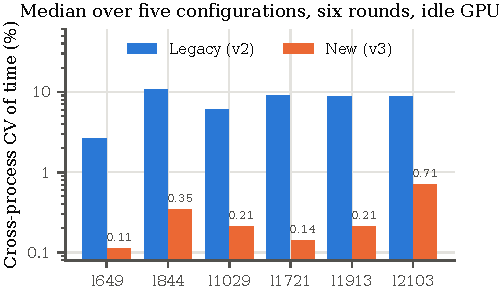
\includegraphics[width=0.48\textwidth]{measurement_cv}
\caption{Cross-process coefficient of variation of kernel time with the legacy (v2) and new (v3) measurement, per LULESH kernel (median over five configurations, six rounds, log scale).}
\label{fig:cv}
\end{figure}
The clean measurements changed the conclusions about individual kernels.
l649 gained 2.54\x{} to 2.66\x{}, which the legacy method had understated as
about 2.1\x{} because it measured during the clock ramp, and l1029 gained
2.41\x{} to 2.43\x{}. For l844, l1721, l1913, and l2103, every earlier winner
measured between 0.98\x{} and 1.004\x{}, so their claimed speedups of
1.22\x{} to 1.47\x{} were noise. This validation varied only the runtime
parameters, and Section~\ref{sec:search} shows that l844 does gain from
launch bounds.

%=============================================================================
\section{Search strategies with clean measurements}
\label{sec:search}

\subsection{Design}
We implemented interchangeable search strategies in \code{RRUtil/Search.py}
and a search loop in \code{Kernel.Search}. All strategies propose points in
the same normalized space and begin with the full launch-bound point, as the
existing BO does. The strategies were the existing GP-UCB with the speedup
objective (\code{bo-speedup}), TPE with the speedup objective
(\code{tpe-speedup}), random search, the existing BO with the energy objective
(\code{bo-energy}), and MOTPE over log speedup and log energy gain
(\code{motpe}). Each configuration was measured with two v3 timing processes
and one metrics replay, which took about 15~s. Runs of the same kernel on the
same GPU shared a measurement cache, which is valid because repeated
measurements now agree within 0.2\%. In total, the study measured 6916
distinct configurations of ten LULESH kernels on five GPUs.

\subsection{Shipped configurations}
Table~\ref{tab:search} shows the true speedup of the configurations that each
strategy shipped. BO, TPE, and MOTPE are statistically indistinguishable, and
random search is 5\% slower, with a 95\% CI that excludes a ratio of 1. The best
known speedups were 2.56\x{} (l649), 2.45\x{} (l1029), 1.55\x{} (l1080),
1.49\x{} (l1201), 1.26\x{} (l844), and 1.10\x{} (l333), and at most 1.05\x{}
for l584, l1721, l1913, and l2103.

\begin{table}[t]
\centering
\caption{Online comparison on ten LULESH kernels, three seeds, 60 proposals.
True speedup is the geometric mean over kernels and seeds of the validated
speedup of the shipped configuration. The CI is a 95\% kernel-clustered
bootstrap of the ratio to \code{bo-speedup}. The last column is the share of
the best known log speedup found after 30 and 60 proposals.}
\label{tab:search}
\begin{tabular}{lrrr}
\toprule
Strategy & True speedup & Ratio to \code{bo-speedup} (95\% CI) & Share at 30 / 60 \\
\midrule
\code{bo-speedup} (existing) & 1.315 & 1 (reference) & 0.73 / 0.86 \\
\code{tpe-speedup} & 1.313 & 0.998 [0.989, 1.008] & 0.80 / 0.88 \\
\code{motpe} & 1.317 & 1.002 [0.992, 1.011] & 0.76 / 0.87 \\
random & 1.248 & 0.949 [0.914, 0.982] & 0.61 / 0.70 \\
\bottomrule
\end{tabular}
\end{table}

TPE found good configurations somewhat earlier than BO
(Figure~\ref{fig:anytime}), never repeated a
configuration (BO repeated 2\% of its proposals), and proposed invalid
configurations less often (0.9\% versus 2.9\%). The winner's curse did not
disappear entirely. On l584 and l2103, which have no real gain, 11 of 120
shipped configurations had measured 1.02\x{} to 1.05\x{} during search but
validated at 0.97\x{} to 0.99\x{}, that is, slower than the baseline. A
tuner should therefore keep the default configuration unless a validation
measurement beats it by a margin.


\begin{figure}[t]
\centering
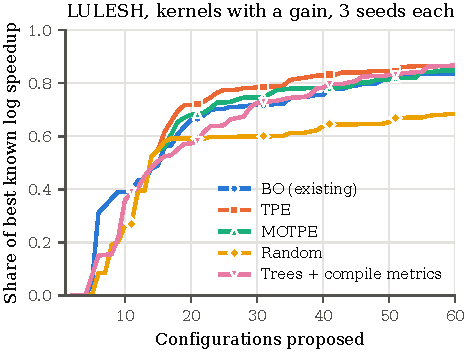
\includegraphics[width=0.48\textwidth]{anytime}
\caption{Share of the best known log speedup found after each proposal, averaged over the LULESH kernels with a gain and three seeds. The first point of every strategy is the full launch-bound configuration, and the model-based strategies start with 15 initial samples. Trees + compile metrics is the \code{trees-meta} strategy of Section~\ref{sec:treesmeta}.}
\label{fig:anytime}
\end{figure}
\subsection{Time and energy}
The time-optimal and energy-optimal configurations differed on every kernel.
Shipping the fastest configuration left 7.6\% of the attainable energy gain
unclaimed (geometric mean), and shipping the most energy-efficient
configuration cost 7.4\% in speed. The trade-off was large on two kernels.
On l333, the fastest configuration gave 1.095\x{} speedup with a 1.17\x{}
energy gain, while another configuration gave a 1.51\x{} energy gain at
1.03\x{} speedup. On l1201, the fastest configuration gave 1.49\x{}, while
the most energy-efficient one gave a 1.83\x{} energy gain at 0.85\x{} speed.
Kernel power ranged from about 40~W to 93~W across configurations, so energy
is not simply proportional to time (Figure~\ref{fig:te}).


\begin{figure}[t]
\centering
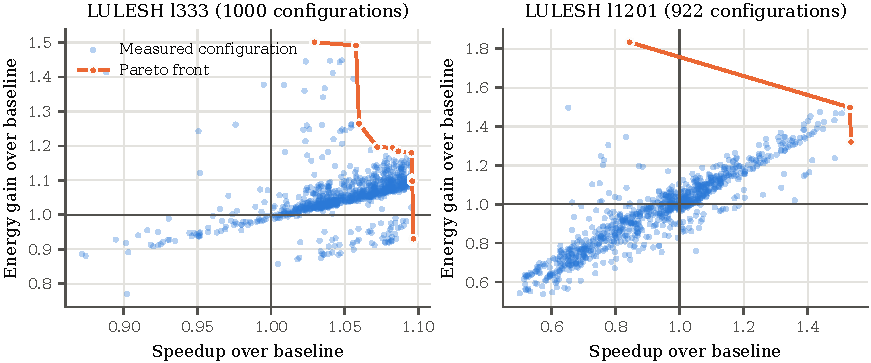
\includegraphics[width=\textwidth]{time_energy}
\caption{Speedup and energy gain of every configuration measured for LULESH l333 and l1201, relative to the baseline, with the Pareto front. On both kernels the fastest configuration is not the most energy-efficient one.}
\label{fig:te}
\end{figure}
Energy-aware search found these trade-offs without losing speed. The
hypervolume reached by each run, relative to the union of all configurations
found, was 0.641 for MOTPE, 0.634 for \code{bo-energy}, 0.623 for
\code{bo-speedup}, 0.618 for TPE, and 0.386 for random search, and MOTPE also
found the highest energy gain (1.384\x{} versus 1.371\x{} for
\code{bo-speedup}). The configuration that MOTPE shipped for speed was as fast
as that of BO. Knowledge of energy therefore does not find faster
configurations, but it does find energy-efficient configurations that a
speed-only search does not report.

\subsection{Predictive value of the metrics with clean data}
With clean data, the launch parameters alone predict the duration well
(median cross-validated Spearman $\rho$ of 0.92). Adding compile-time
registers and spills raises it to 0.95, adding the measured occupancy, branch
efficiency, loads, and stores raises it to 0.96, and adding power raises it to
0.98. Most of the improvement occurs among the best configurations, where
$\rho$ within the top 20\% rises from 0.38 with launch parameters alone to
0.55 with compile-time features and 0.72 with measured metrics. Registers and
occupancy track duration closely on the register-bound kernels (absolute
Spearman $\rho$ of 0.7 to 0.9 on l844, l1080, l1721, and l1913).

%=============================================================================
\section{Metrics that vary with the launch configuration}
\label{sec:metrics}

\subsection{Extended metric collection}
We extended the plugin so that \code{LIBOMPTARGET\_RR\_EXTRA\_METRICS} appends
perfworks metrics to its fixed set of eight, and so that every metric value is
printed to standard output. The tuner passes a list that we validated against
the 1684 metrics that the T4 supports: DRAM and SM throughput as a percentage
of peak, L2 sectors and hit rate, L1 hit rate, global load sectors,
instructions executed, FP64 instructions and pipe utilization, active cycles,
active threads per instruction, the average warp latency stalled on long
scoreboard dependencies (memory), and GPU time. Each configuration's database
entry stores these metrics and the SM clock observed during timing. The extra
counters add about 0.2~s per metrics replay.

\subsection{What varies and what explains performance}
DRAM traffic varied by up to 8\x{} across launch configurations, while the
load request counts stayed constant. On the two kernels with the largest
gains, l649 and l1029, the Spearman correlation between duration and DRAM
sectors read was 0.98 and 0.99. Their 2.5\x{} speedup is a traffic reduction,
because the best configurations read 63\% less data from DRAM and raised the
L2 hit rate from 33\% to 78\%. On the register-bound kernels (l844, l1080,
l1721, l1913), local (spill) loads tracked duration ($\rho$ of 0.65 to 0.78),
and so did achieved occupancy on l844 ($\rho$ of 0.74). On l844, the full
block configuration read four times as many DRAM sectors as the baseline
while executing the same number of load instructions.
Figure~\ref{fig:dram} shows both metrics against kernel time.


\begin{figure}[t]
\centering
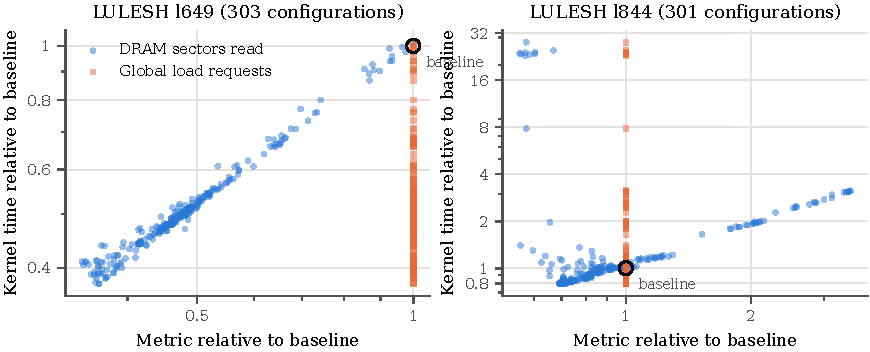
\includegraphics[width=\textwidth]{dram_traffic}
\caption{Kernel time against DRAM sectors read (blue) and global load requests (orange), both relative to the baseline, for every configuration of LULESH l649 and l844 measured with the extended metrics. Load requests do not change with the launch configuration, while DRAM traffic varies widely and, on l649, determines the time.}
\label{fig:dram}
\end{figure}
\subsection{A search that uses compile-time metrics}
\label{sec:treesmeta}
Registers and spills are known before a configuration runs, because they
depend only on the launch bounds. We therefore compiled each kernel once for
every (\code{MaxThreads}, \code{MinTeams}) pair, 119 pairs in about one minute
(0.4~s each), and recorded the registers and spills reported by \code{ptxas}.
From this table, we compute theoretical occupancy, waves, and tail efficiency
for any configuration. We compared two strategies that share an ExtraTrees
surrogate with EI over random and local candidates. \code{trees-config} uses
only the launch parameters, and \code{trees-meta} adds the compile-time
features and never proposes a configuration whose registers times threads
exceed the 65536-register limit of a block.

Overall, \code{trees-meta} tied the other strategies (true speedup 1.303
versus 1.306 for \code{bo-speedup}, ratio 0.998 with CI [0.961, 1.042]).
Per kernel, however, the effect was large and consistent across seeds. It
improved on \code{trees-config} by 8.1\% on l1201, 5.4\% on l1080, and 1.0\%
on l844, on all three seeds each, and it shipped the best configuration of
any strategy on l1201 (1.48\x{} versus 1.29\x{} for BO). It was worse by
6.2\% on l649 and 9.2\% on l1029 (Figure~\ref{fig:meta}). The compile-time features help where
registers limit performance and mislead the surrogate where the bottleneck is
cache locality, because they add input dimensions that do not explain the
duration of those kernels.


\begin{figure}[t]
\centering
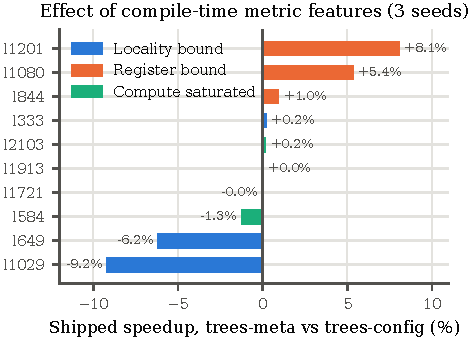
\includegraphics[width=0.48\textwidth]{meta_effect}
\caption{Change in the validated speedup of the shipped configuration when the tree surrogate also uses compile-time features (\code{trees-meta}) instead of launch parameters alone (\code{trees-config}), per LULESH kernel, geometric mean over three seeds, colored by bottleneck class.}
\label{fig:meta}
\end{figure}
\subsection{Early stopping}
We replayed the 120 completed speed-objective searches under candidate
stopping rules. Rules that stop after a fixed number of proposals without a
1\% or 2\% improvement saved about 40\% of the budget but lost more than 2\%
of the final gain in 14 to 15 runs (worst 0.76 of the final speedup),
because improvements often arrive late. Stopping when the best speedup after
30 proposals is below 1.03\x{} saved 15\% but cut off searches of l844 and
l1201 that later found real gains. Baseline metrics separated the kernels
cleanly. Every kernel with at most 1.05\x{} to gain (l584, l1721, l1913,
l2103) had a baseline SM throughput of 83\% to 88\% with the FP64 pipe at
84\% to 88\%, and every kernel with a real gain had at most 51\%. A DRAM
bandwidth ceiling is the wrong test, because l649 and l1029 ran at 85\% to
88\% of peak DRAM bandwidth yet gained 2.5\x{} by moving less data. We
added the rule as an option that is disabled by default
(\code{RR\_SATURATED\_SM\_PCT} and \code{RR\_SATURATED\_BUDGET}).

%=============================================================================
\section{Bottleneck-specific objectives}
\label{sec:targets}

We asked whether the search should switch its objective once it knows the
kernel's bottleneck, for example to DRAM traffic for a locality-bound kernel
or to spills and occupancy for a register-bound kernel. We distinguish the
\emph{steering} objective, which guides the surrogate, from the \emph{shipping}
criterion, which selects the result. Every configuration's duration is
measured anyway, so every strategy below ships the configuration with the best
measured speedup, and the steering objective only changes which
configurations are tried.

\subsection{Traffic as an objective}
Minimizing DRAM traffic is a good proxy only on locality-bound kernels. On
l1029, the configuration with the least traffic ran at 2.42\x{} against a
best of 2.43\x{}, and on l649 at 2.44\x{} against 2.67\x{}. On the
register-bound kernels l844 and l1080, it ran at 0.04\x{} and 0.05\x{},
because the least traffic comes from nearly serial configurations. Traffic
can therefore guide a search but must not select the result.

The least-traffic configuration also had near-optimal energy on
locality-bound kernels (energy gains of 2.42\x{}, 2.40\x{}, and 1.15\x{}
against best values of 2.69\x{}, 2.48\x{}, and 1.16\x{} on l649, l1029, and
l333). Their baselines and their least-traffic configurations both drew about
69~W, at the power limit, so energy followed time. On l333, the least-traffic
configuration used less energy than the fastest one, which used 10\% more
energy than the baseline. On register-bound kernels, the least-traffic
configurations used 13\x{} to 17\x{} more energy than the baseline, because
they drew less power (47~W to 48~W) but ran about 20\x{} longer.

\subsection{Simulated comparison}
We simulated pool-based searches on the roughly 300 configurations per kernel
that carried the extended metrics, with an ExtraTrees surrogate, 15 random
initial samples, and 20 seeds. Kernels were classified from baseline metrics
as compute saturated, locality bound, or register bound
(Section~\ref{sec:adaptive}). The class-specific steering objectives were
DRAM traffic for locality-bound kernels and the mean of standardized spill
loads and occupancy for register-bound kernels, either alone or mixed in
equal weight with standardized log speedup. A data-driven variant chose,
after the initial samples, the metric with the strongest rank correlation
with duration.

On locality-bound kernels, no steering objective improved on speedup
(0.976 versus 0.977 of the attainable gain at 30 evaluations), because
traffic and duration are nearly the same signal there (Spearman $\rho$ of
0.99). On register-bound kernels, the condition metric mixed with speedup
reached a given quality sooner (0.978 versus 0.963 at 30 evaluations, and
0.993 versus 0.984 at 45), and by 60 evaluations all variants converged.
The condition metric alone was no better than speedup. The data-driven
variant chose traffic on 56 of 60 locality-bound seeds but often chose the
wrong metric on register-bound kernels, for example the L2 hit rate on
l1201, which made it worse. A fixed mixture of traffic and speedup for all
kernels improved the overall share of attainable gain from 0.920 to 0.936 at
30 evaluations and from 0.965 to 0.979 at 60. The pool contained only
configurations that earlier tree-based searches had chosen, and every
strategy came close to its best, which compresses the differences.

%=============================================================================
\section{A bottleneck-adaptive tuning pipeline}
\label{sec:adaptive}

\subsection{Pipeline}
The results above suggest choosing the search strategy by bottleneck class.
The \code{adaptive} strategy in \code{Kernel.Search} works as follows. First,
it measures the baseline three times with metrics and takes the median of
each metric. Second, it classifies the kernel with the following rules, in
order. A kernel is \emph{compute saturated} if its SM throughput exceeds
80\% of peak and its DRAM throughput is below 70\%, \emph{locality bound} if
its achieved occupancy exceeds 80\% and its DRAM throughput exceeds 70\%,
and \emph{register bound} if it has local-memory loads or an occupancy below
60\%. Third, it searches the speedup objective with the strategy that suited
the class. Compute-saturated kernels get TPE with the budget cut to 15
proposals. Register-bound kernels get \code{trees-meta} with a steering
objective that mixes speedup with spills and occupancy, relabeled at every
step. All other kernels get TPE.

\subsection{Measurement problems found while deploying the pipeline}
The classification exposed two further measurement problems. First, the
metrics replay profiled a single cold launch. Counts such as DRAM sectors do
not depend on the clock, but utilization percentages do, because at a low SM
clock memory looks relatively fast and the SM looks busy. The GPU time of the
same baseline varied by up to 2\x{} (l1721: 9.6~ms to 18.6~ms), and the SM
utilization of l844 varied from 48\% to 87\%, which made two early runs
classify l844 as compute saturated. We added
\code{LIBOMPTARGET\_RR\_METRICS\_WARMUP\_MS}, which launches the kernel for
1~s before profiling, and tagged warm metrics so that the steering objective
ignores cold ones. With the warm-up, every one of 17 kernels received the
same class in four repeated measurements. Second, l844, the kernel with the
highest power, can still be throttled by the 70~W limit during the profiling
passes, which raised its SM utilization to 88\% in one warm sample. We
therefore require low DRAM throughput for the compute-saturated class, which
the LULESH data support (compute-saturated kernels had DRAM throughput of at
most 66\%, and l844 had 69\% to 88\%), and classify from the median of three
samples. Neither change affects any miniFE kernel. We discarded the two
aborted attempts and kept their files for reference.

\subsection{Classes}
Figure~\ref{fig:classes} places every kernel by its warm baseline metrics.
The rules classified the LULESH kernels l333, l649, and l1029 as locality
bound, l844, l1080, and l1201 as register bound, and l584, l1721, l1913, and
l2103 as compute saturated. They classified the miniFE kernels l157, l169,
l205, l210 (vector operations at 85\% to 89\% of peak DRAM bandwidth) and
l521 (sparse matrix-vector product at 91\%) as locality bound, and l254 and
l290 as register bound. The miniFE kernels l254 and l290 and the LULESH
kernel l1201 are reductions. Their local-memory loads (26496 in each case)
come from the OpenMP runtime's reduction code rather than from register
pressure, so "register bound" is a misnomer for them, although the register
steering suited them (Table~\ref{tab:adaptive}).


\begin{figure}[t]
\centering
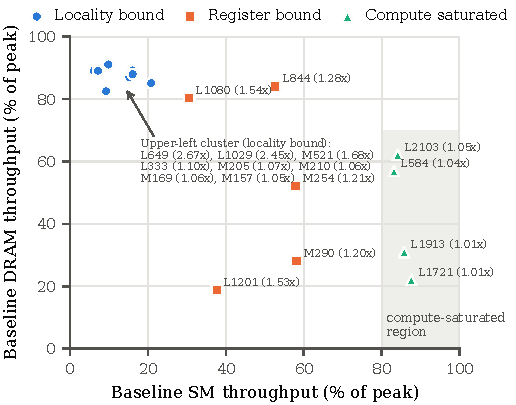
\includegraphics[width=0.48\textwidth]{classes}
\caption{Warm baseline SM and DRAM throughput of the ten LULESH (L) and seven miniFE (M) kernels, colored by the class that the rules assign, with the best known speedup in parentheses. Compute-saturated kernels (shaded region) had nothing to gain.}
\label{fig:classes}
\end{figure}
\subsection{Results}
Table~\ref{tab:adaptive} reports the true speedups. On LULESH, the pipeline
shipped the fastest configurations overall while measuring 30\% fewer
configurations (1260 versus 1800), because it stopped early on
compute-saturated kernels. Its gain over BO was within noise (ratio 1.010,
CI [0.986, 1.043]). On the register-bound class, it nearly matched
\code{trees-meta}, and on the locality-bound class it matched TPE, as
designed. On the compute-saturated class, its short searches shipped slightly
slower configurations (0.992\x{}, with l1913 at 0.969\x{}), which a rule that
keeps the default configuration for these kernels would avoid.

On the seven held-out miniFE kernels, the pipeline improved on BO by 1.3\%
(CI [0.9998, 1.028]) and on TPE by 0.7\% (CI [1.000, 1.018]), entirely
through the two reduction kernels, where it shipped 1.056\x{} and 1.081\x{}
against 1.018\x{} and 1.066\x{} for TPE. On the five locality-bound miniFE
kernels, all strategies were within 0.3\% of each other. The miniFE kernel
l169 has two seeds instead of three, because another job occupied its GPU
during the third. Over all 17 kernels, the pipeline shipped the fastest
configurations of any strategy (1.242\x{} against 1.228\x{} for BO,
1.229\x{} for TPE, and 1.237\x{} for \code{trees-meta}), although none of
these differences is statistically resolved (ratio to BO 1.011, CI [0.995,
1.031]).

\begin{table}[t]
\centering
\caption{True speedup of shipped configurations by bottleneck class
(geometric mean over kernels and three seeds; two seeds for miniFE l169).}
\label{tab:adaptive}
\begin{tabular}{llrrrr}
\toprule
Application & Class (kernels) & \code{bo-speedup} & \code{tpe-speedup} & \code{trees-meta} & \code{adaptive} \\
\midrule
\multirow{4}{*}{LULESH}
& Locality bound (3) & 1.866 & 1.840 & 1.752 & 1.839 \\
& Register bound (3) & 1.306 & 1.313 & 1.398 & 1.385 \\
& Compute saturated (4) & 1.001 & 1.002 & 1.000 & 0.992 \\
& All (10) & 1.307 & 1.304 & 1.309 & 1.320 \\
\midrule
\multirow{3}{*}{miniFE}
& Locality bound (5) & 1.163 & 1.163 & 1.161 & 1.163 \\
& Register bound (2) & 1.023 & 1.042 & 1.079 & 1.068 \\
& All (7) & 1.119 & 1.125 & 1.136 & 1.134 \\
\bottomrule
\end{tabular}
\end{table}

%=============================================================================
\section{Further avenues for searching faster}
\label{sec:efficiency}

We estimated the potential of further techniques on the 13259 configurations
measured with v3 timing, using exact measurements where possible and an
ExtraTrees model trained on each kernel's measurements as an approximate
oracle otherwise. We also surveyed the literature on sample-efficient
autotuning.

\subsection{Cost of one evaluation}
We timed each kind of replay process on three idle GPUs for two LULESH
kernels and one miniFE kernel, three times each. A process that only loads
the recording and launches the kernel once took 2.9~s to 3.9~s, so process
start-up and loading the recorded memory form a fixed floor. The 1~s warm-up
and ten timed launches added about 1.1~s, the energy window added 0.3~s, and
a warmed metrics replay took 5.5~s to 6.5~s (4.1~s to 5.0~s without the
warm-up). One configuration in our studies therefore cost about 0.4~s of
compilation, two timing processes of about 4.4~s each, and one metrics
process of about 5.5~s, close to the observed 15~s (Figure~\ref{fig:cost}). About 60\% of that
time is the fixed per-process floor, paid three times. Two changes follow. First,
screening a candidate with one timing process and no metrics replay costs
about 4.8~s, a third of a full evaluation, and with 0.23\% noise a single
process ranks candidates reliably. Second, evaluating several runtime
configurations inside one replay process would pay the floor and the warm-up
once, which would reduce the cost of a runtime-only variant to roughly one
second. Section~\ref{sec:batch} implements and evaluates this change.


\begin{figure}[t]
\centering
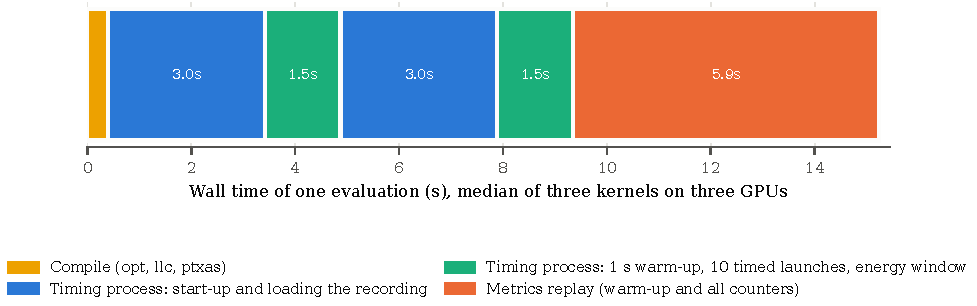
\includegraphics[width=\textwidth]{cost_breakdown}
\caption{Wall time of one evaluation, built from the measured median cost of each replay process (two LULESH kernels and one miniFE kernel on three GPUs) and the measured compile time.}
\label{fig:cost}
\end{figure}
The same measurements show that GPUs of the node can share a search. The
median durations of the two LULESH kernels agreed within 0.2\% to 0.3\%
across three GPUs. The 0.95~ms miniFE kernel differed by 2.5\% between GPUs,
so short kernels need a baseline measured on each GPU. A shorter warm-up of
0.5~s with five timed launches gave the same medians as the default within
0.1\% on the LULESH kernels but differed by 2.3\% on the short kernel, so we
keep the 1~s default.

\subsection{Redundancy in the launch bounds}
The 119 launch-bound pairs of a kernel compiled to only 1 to 8 distinct
binaries (distinct register and spill counts), and 10 of 17 kernels had at
most 2. Permutation importance on log duration showed that the number of teams
explained 85\% to 99\% of the variance on locality-bound kernels and
reductions, while the launch bounds explained 64\% to 85\% on l844, l1080,
and l1913. Exact duplicates, two proposals with the same binary and the same
runtime parameters, were rare in real searches (0\% to 4\% of measured
configurations), because \code{NumTeams} is nearly continuous. The redundancy
therefore costs the surrogate, which must learn over two dimensions that
rarely change the binary, more than it costs repeated measurements. A
reparameterization into a categorical binary class, \code{NumThreads}, and
the teams fraction would remove it. Restricting the search to
\code{MinTeams} = 1 kept 99.9\% of the best speedup on average (at least
98.3\%), and additionally tying \code{NumThreads} to \code{MaxThreads} kept
96.7\% on average but only 85\% to 89\% on the reductions, so such
restrictions should depend on the class.

\subsection{Priors from the structure of good configurations}
Good configurations shared structure that depended on the class. Of the best
5\% of configurations of locality-bound kernels, 89\% used a teams fraction of
at least 0.9 (one iteration per thread), against 36\% of all measured
configurations. Of the best configurations of the register-bound class, which
here includes the reductions, 60\% used a teams fraction below 0.25. All of
the best configurations of compute-saturated kernels used at most 256 threads
per team. Prior-guided BO methods such as $\pi$BO~\cite{hvarfner2022pibo} and
BOPrO~\cite{souza2021bopro} can use such priors while limiting the damage of
a wrong prior.

\subsection{Transfer across kernels}
We built portfolios of initial configurations from the best configurations of
other kernels, expressed with the teams fraction so that they transfer across
trip counts, and selected them greedily to maximize the mean share of
attainable gain over the source kernels. Evaluated on each target kernel with
leave-one-kernel-out selection, five portfolio configurations reached 0.42 of
the attainable gain (0.48 when drawn only from kernels of the same class),
against 0.13 for five random configurations, 0.28 for five Sobol points, and
0.38 for ten hand-written heuristic configurations. With ten configurations,
the portfolio reached 0.56 against 0.39 for random and 0.45 for Sobol
(Figure~\ref{fig:init}). The
literature reports similar effects. A Gaussian copula model of earlier tuning
results reached 64\% of peak performance on the first evaluation~\cite{randall2023copula},
and on GPUs, the important parameters transfer across devices while the best
values do not~\cite{torring2023benchmark}.


\begin{figure}[t]
\centering
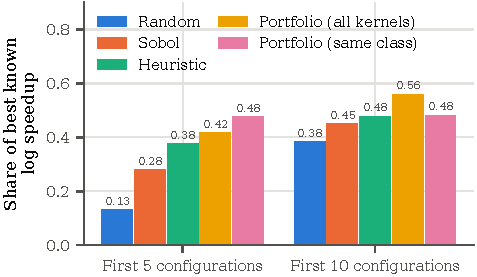
\includegraphics[width=0.48\textwidth]{initial_designs}
\caption{Best-of-$k$ share of the best known log speedup for initial designs, averaged over target kernels with a gain, estimated with a surrogate trained on each target kernel's measurements. Portfolios are selected from other kernels only (leave one kernel out). The heuristic design has ten hand-written configurations.}
\label{fig:init}
\end{figure}
\subsection{Pruning and early termination}
Pruning before measurement had limited value. Rejecting configurations that
spill when a launch bound without spills exists removed 14\% of the measured
configurations and only 0.4\% of the best 5\%, but it would have removed the
best configuration of l584. Combining it with rules on predicted occupancy and
waves removed 75\% of the configurations slower than 0.8\x{} but also 14\% of
the best 5\% and the best configuration of four kernels. In realistic TPE
searches, 16\% to 18\% of measured configurations ran slower than 0.8\x{} the
baseline. Abandoning such a configuration after its first timed launch would
reduce the wall time per configuration by about 11\%.

\subsection{Related techniques from the literature}
The literature suggests several further techniques. Multi-fidelity methods
such as BOHB~\cite{falkner2018bohb}, GPTuneBand~\cite{zhu2022gptuneband}, and
racing~\cite{lopezibanez2016irace} spend full evaluations only on promising
candidates. With 0.23\% noise, one short timing replay without the metrics
replay could screen candidates. Cost models rank many candidates before
measuring, as in Ansor~\cite{zheng2020ansor}, and BaCO adds a learned
feasibility model for constrained compiler spaces~\cite{hellsten2023baco}.
Filipovi\v{c} et al.\ used hardware counters to steer the search of GPU
kernel tuning~\cite{filipovic2022counters}, which is the closest published
analogue to our metric-aware search. Schoonhoven et al.\ compared 16
optimizers on GPU tuning problems and found dual annealing best at budgets of
at most 200 evaluations~\cite{schoonhoven2023benchmark}. Automatic
termination based on the gap between a regret bound and the measurement noise
gives a principled stopping rule~\cite{makarova2022termination}. Asynchronous
batch proposals, such as Optuna's constant-liar TPE, can use several GPUs at
once~\cite{ginsbourger2010kriging}. Large language models have been used to
propose configurations and priors, with a vendor report of 9.8\x{} fewer
configurations for comparable results on Helion kernels~\cite{helion2026llm}.


\subsection{Online evaluation of four avenues}
\label{sec:avenues}
We implemented the four most promising avenues and tested each one online
against its natural baseline on 13 kernels, the six LULESH kernels with a
gain (l333, l649, l844, l1029, l1080, l1201) and all seven miniFE kernels,
with three seeds each. The compute-saturated kernels were excluded, because
they have nothing to gain. Every phase re-measured the shipped configurations
of the avenue and of its baseline together with the baseline configuration in
five randomized rounds. Runs of a kernel shared its measurement cache, and the
two short miniFE kernels l169 and l254 used a fresh cache when they moved to
another GPU, because their timings can differ by 2.5\% between GPUs. To give
the cheaper evaluations of multi-fidelity search a fair comparison, we measure
progress against a nominal cost (14.6~s for a full evaluation, 4.4~s for a
screening evaluation, and 9.85~s for promoting a screened configuration to a
full evaluation, Figure~\ref{fig:cost}), and we charge cache hits their
nominal cost.

The four avenues were as follows. First, \emph{multi-fidelity screening}
(\code{tpe-mf}) evaluates every TPE proposal with one timing process and no
energy window or metrics replay, within the nominal cost of 60 full
evaluations, and then fully measures the five best screened configurations
and ships the best of them. A run thus screened 187 configurations on
average. Second, the \emph{portfolio warm start} (\code{tpe-portfolio})
replaces TPE's first ten proposals with the best configurations of other
kernels, taking kernels of the same class first and mapping each
configuration to the target trip count through its teams fraction. Third,
the \emph{transfer cost model} (\code{transfer-model}) fits an ExtraTrees
model on the measurements of all other kernels plus the target kernel's own,
which receive 20 times the weight, over features that do not depend on the
kernel (threads, teams fraction, registers, spills, theoretical occupancy,
waves, tail efficiency, and bottleneck class). It ranks a candidate set with
one launch bound per distinct binary, every warp multiple of threads, and 28
teams fractions, never proposes the same binary and launch twice, and uses
expected improvement from the first proposal without random initial samples.
Fourth, the \emph{prior-guided search} (\code{trees-prior}) multiplies the
expected improvement of the \code{trees-config} surrogate by a prior raised to
the power $\beta/n$, as in $\pi$BO~\cite{hvarfner2022pibo}, with $\beta = 10$
and $n$ the number of observations. The prior is a Gaussian kernel density
estimate over the best 5\% of configurations of other kernels of the same
class, mixed with a uniform density of weight 0.1, and the initial samples are
drawn from it. All transfers leave the target kernel out.

Table~\ref{tab:avenues} and Figure~\ref{fig:avenues} show the results. Every
avenue found good configurations much earlier than its baseline, and every
avenue shipped faster configurations on average. The portfolio and the
transfer cost model improved the shipped speedup by 1.2\% and 1.9\%, and
their confidence intervals exclude a ratio of 1. Multi-fidelity screening
reached 0.74 of the attainable gain within the cost of ten full evaluations,
against 0.42 for TPE, but on the 0.95~ms miniFE kernel l254 it shipped a
configuration that validated at 0.969\x{}, because a single timing process
of a short kernel is noisier than the median of two. The prior-guided search
gave the most lasting improvement in progress, 0.92 against 0.88 of the
attainable gain after 60 evaluations. The early advantage of the portfolio
and of the transfer cost model narrowed by 60 evaluations, which suggests that
they help most when the budget is small.

\begin{table}[t]
\centering
\caption{Online evaluation of four avenues on 13 kernels (three seeds each).
The shipped speedup is the geometric mean ratio of the validated speedup of
the avenue's shipped configuration to that of its baseline, with a 95\%
kernel-clustered bootstrap CI. Progress is the share of the best known log
speedup found within a nominal cost of 10 and 60 full evaluations.}
\label{tab:avenues}
\small
\setlength{\tabcolsep}{4pt}
\begin{tabular}{llrrr}
\toprule
Avenue & Baseline & Shipped ratio (95\% CI) & Better / worse & Progress at 10 / 60 \\
\midrule
Multi-fidelity screening & TPE & 1.014 [0.998, 1.031] & 5 / 1 & 0.74 / 0.91 (0.42 / 0.87) \\
Portfolio warm start & TPE & 1.012 [1.002, 1.023] & 4 / 1 & 0.59 / 0.86 (0.44 / 0.80) \\
Transfer cost model & TPE & 1.019 [1.003, 1.044] & 5 / 1 & 0.70 / 0.82 (0.50 / 0.80) \\
Transfer cost model & \code{trees-meta} & 1.009 [0.991, 1.030] & 3 / 3 & 0.70 / 0.82 (0.49 / 0.83) \\
Prior-guided search & \code{trees-config} & 1.010 [0.999, 1.021] & 6 / 2 & 0.71 / 0.92 (0.50 / 0.88) \\
\bottomrule
\end{tabular}
\end{table}

\begin{figure}[t]
\centering
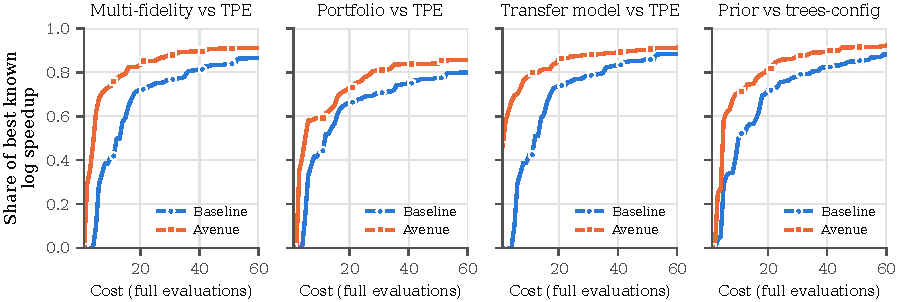
\includegraphics[width=\textwidth]{avenues}
\caption{Share of the best known log speedup found within a nominal cost,
expressed in full evaluations, for each avenue and its baseline, averaged over
13 kernels and three seeds. Each panel uses its own phase's measurements, so
the baselines differ slightly between panels.}
\label{fig:avenues}
\end{figure}

\subsection{In-process batch replay}
\label{sec:batch}
We extended the replay tool so that one process evaluates many launch
configurations. The option \code{--batch} reads one pair of team and thread
counts per line and replays every pair, printing a marker before each one.
The runtime allocates the recorded memory region once per process and restores
the recorded inputs before each configuration, so that every configuration
starts from the recorded state and the recorded pointer arguments remain
valid. With \code{LIBOMPTARGET\_RR\_DEVICE\_RESTORE}, the runtime keeps a
copy of the inputs on the device after the first transfer and restores from it
with a device-to-device copy instead of re-sending 2~GB to 3~GB from host
memory. The plugin performs the full 1~s warm-up only for the first
configuration of a process and re-warms for 100~ms before later ones. In the
tuner, \code{Kernel.sample\_batch} compiles each distinct binary once (launch
bounds with the same registers and spills share a binary) and evaluates its
configurations in one process, and it continues in a new process when a
configuration makes the replay fail. The \code{tpe-batch} strategy asks TPE for
16 proposals at a time, using Optuna's constant-liar mode so that pending
proposals are not repeated, groups them by binary, and screens each group in
one batch replay. As in multi-fidelity screening, the five best screened
configurations then receive the standard full measurement, and the best of
them is shipped.

Batch replay cost 0.48~s to 0.58~s per configuration on three kernels, against
3.7~s to 4.7~s with one process per configuration, and 0.87~s to 1.13~s when
the inputs were restored from host memory. On the 7~ms kernel l649, batch
timings matched single-process timings within 0.2\% (median). On the short
kernels l2103 (1.7~ms) and miniFE l254 (0.95~ms), batch timings were 1\% to
1.5\% slower, because a batch keeps the GPU under sustained load, which holds
the T4 at its 70~W limit. NVML reported an SM clock of 1380~MHz to 1455~MHz with
the power cap active during a batch, against 1590~MHz in short single-process
replays. Batch screens therefore rank candidates, and the shipped
configuration is chosen with the standard measurement.

We compared \code{tpe-batch} with multi-fidelity screening that uses one
process per screen, both under the same real wall-clock budget of 300~s per
run and without the measurement cache, on l649, l1201, l844, and miniFE l290
and l521, with three seeds each. Table~\ref{tab:batch} shows the result. Batch
screening evaluated 239 configurations per run against 36, reached a better
configuration in 30~s than one process per screen reached in 2 minutes, and
shipped configurations that were 6.8\% faster (CI [1.017, 1.138]). It was also
5.3\% faster (CI [1.011, 1.105]) than TPE with 60 full evaluations, which had
three times the nominal budget and the cache.

\begin{table}[t]
\centering
\caption{Batch screening against one process per screen, both with a real
wall-clock budget of 300~s per run and no measurement cache (five kernels,
three seeds). Shipped speedups are validated; the best screened speedups are
geometric means of each run's own screens.}
\label{tab:batch}
\small
\begin{tabular}{lrrrr}
\toprule
Strategy & Screens per run & Best screen at 30 / 60 / 120~s & Shipped speedup \\
\midrule
Multi-fidelity, one process per screen & 36 & 1.111 / 1.251 / 1.406 & 1.443 \\
Batch screening (\code{tpe-batch}) & 239 & 1.343 / 1.475 / 1.517 & 1.541 \\
TPE, 60 full evaluations (cached) & 60 & --- & 1.463 \\
\bottomrule
\end{tabular}
\end{table}


\subsection{Batch screening combined with the other avenues}
\label{sec:combinedbatch}
We combined batch screening with the portfolio warm start, the transfer cost
model, the prior, and a convergence-based stop in one strategy,
\code{combined-batch}. The transfer cost model proposes 16 candidates per
batch, namely those with the highest prior-weighted expected improvement that
differ in binary or launch configuration from each other and from everything
evaluated so far, and the first batch is filled with the cross-kernel
portfolio. Each batch is screened with batch replay. The search stops when the
largest expected improvement predicted by the model, in log speedup, falls
below 0.002, which is the measurement noise, or when the 300~s budget is
spent. The best screens are then promoted to the standard measurement. We
compared it with \code{tpe-batch} and with the same combination without the
stop (\code{combined-batch-nostop}), on the five kernels of
Section~\ref{sec:batch} with three seeds, without the measurement cache.

Table~\ref{tab:combinedbatch} shows the result. The combination shipped
configurations as fast as \code{tpe-batch} (ratio 0.996, CI [0.975, 1.017])
and 4.4\% faster than TPE with 60 full evaluations (CI [1.006, 1.093]), while
using 27\% less wall time and 42\% less search time. The benefit comes from the
convergence stop. Without the stop, the combination was no better than
\code{tpe-batch} (ratio 0.987) and worse on l649 (2.32\x{} against 2.59\x{}),
because the transferred model and the prior steer the search toward regions
that suit other kernels, while TPE explores well on its own once screens are
cheap. The stop fired in 12 of 15 runs, after 18~s on l1201 and 80~s to 150~s
on l649, l844, and l290. The three runs that used the whole budget were on
miniFE l521. On l1201 the stop came slightly early (1.444\x{} against
1.473\x{} for \code{tpe-batch}).

Promotions now account for half of the remaining time, at about 20~s each. The
configuration that \code{combined-batch} shipped was its best screen in all 15
runs, so promoting two configurations would ship the same results in about
148~s per kernel, half the time of \code{tpe-batch} and about one sixth of the
nominal time of TPE with 60 full evaluations. \code{tpe-batch} shipped its third
or fourth best screen in 6 of 15 runs, so it needs more promotions, because
batch timings of short kernels are noisier.

\begin{table}[t]
\centering
\caption{Batch screening combined with the transfer cost model, portfolio,
prior, and convergence stop (five kernels, three seeds, no cache, real wall
time including five promotions).}
\label{tab:combinedbatch}
\small
\begin{tabular}{lrrr}
\toprule
Strategy & Shipped speedup & Wall time per run & Screens \\
\midrule
TPE, 60 full evaluations (cached) & 1.469 & about 15 min nominal & 60 \\
\code{tpe-batch} & 1.540 & 288~s & 239 \\
\code{combined-batch-nostop} & 1.520 & 290~s & 239 \\
\code{combined-batch} & 1.534 & 210~s (148~s with two promotions) & 112 \\
\bottomrule
\end{tabular}
\end{table}


%=============================================================================
\section{Discussion and recommendations}
\label{sec:discussion}

The answer to the first question is that knowledge of all metrics helps, but
only through metrics that vary with the launch configuration. DRAM traffic
and L2 hit rate explain the large gains on locality-bound kernels, registers,
spills, and occupancy explain the register-bound kernels, and SM and FP64
saturation of the baseline predicts when a kernel has nothing to gain.
Energy as now measured reveals real energy savings that a speed-only search
misses, and the global load and store request counts explain nothing. The
answer to the second question is that, once measurements are clean, the
choice among model-based search algorithms matters little, while the choice
of model features, initial design, budget, and stopping rule matters more.

We recommend the following changes to the tuner, in order of expected
benefit per unit of effort.
\begin{enumerate}
\item Screen candidates with in-process batch replay (Section~\ref{sec:batch}),
  which made each screen about eight times cheaper, stop when the model's
  expected improvement falls below the measurement noise, and confirm the
  finalists with the standard measurement (Section~\ref{sec:combinedbatch}).
\item Keep the v3 measurement, including the metrics warm-up, the exclusivity
  guard, and validation of the shipped configuration against the baseline,
  with the default kept when the validated gain is below about 2\%.
\item Classify the kernel from warm baseline metrics, stop early on
  compute-saturated kernels, and choose the surrogate features by class.
\item Seed the search with a portfolio of configurations transferred from
  similar kernels, or rank candidates with a cost model transferred across
  kernels, instead of random initial samples (Section~\ref{sec:avenues}).
\item Screen candidates with a single short timing replay and fully measure
  only the best few, keeping the default configuration when a short kernel's
  promoted winner does not beat it, and reparameterize the launch bounds as a
  categorical binary class.
\item Use the best configurations of same-class kernels as a prior for the
  acquisition function, which kept the largest progress advantage in our
  tests.
\item Use MOTPE when energy matters, because it finds the time-energy
  trade-off at no cost in speed.
\end{enumerate}

\subsection{Limitations}
A limitation of this study is that it used one GPU model, the T4, which has a
low power limit and weak FP64 throughput, which affects both the bottleneck
classes and the time-energy trade-off. The applications were two proxy
applications with one recorded input each. The classification thresholds were
derived from the ten LULESH kernels, and miniFE is the only held-out test.
The offline estimates in Sections~\ref{sec:offline}, \ref{sec:targets},
and~\ref{sec:efficiency} use pools of configurations that earlier searches
chose, which bias them toward the regions those searches visited, and the
surrogate oracle used for the transfer estimates extrapolates beyond the
measured configurations. Repeated launches of one configuration in timing
mode reuse modified buffers, which can change the behavior of kernels that
update their inputs, although batch replay restores the inputs between
configurations.

%=============================================================================
\section{Reproducibility}
\label{sec:repro}

The code changes are on branch \code{measurement-v3} of the \code{openmp-rr}
repository: commit \code{a6a4418ce} (v3 measurement), commit \code{0d0b53d39}
(search strategies and the NVML device mapping fix), commit \code{5ee0f82bd}
(extended metrics, metric-aware search, early stopping), and commit
\code{865c4657b} (metrics warm-up and the adaptive pipeline). Each experiment directory
under \code{experiment-archives/} contains its scripts, logs, exit codes, and
a \code{RESULTS.md} file: \code{optimizer-study-2026-10-09}
(Section~\ref{sec:offline}), \code{measurement-fix-2026-10-09}
(Section~\ref{sec:measurement}), \code{search-study-2026-10-09}
(Section~\ref{sec:search}), \code{metric-search-2026-10-10}
(Sections~\ref{sec:metrics} and~\ref{sec:targets}),
\code{adaptive-2026-10-10} (Section~\ref{sec:adaptive}), and
\code{search-efficiency-2026-10-10} (Section~\ref{sec:efficiency}), and
\code{avenues-online-2026-10-11} (Section~\ref{sec:avenues}), and
\code{batch-replay-2026-10-11} (Section~\ref{sec:batch}). Batch replay is
commit \code{b6fd8c751}, and the combined strategy with the convergence stop is
commit \code{6f5c4c482} (\code{combined-batch-2026-10-12}).
Optuna~3.6.1 is not part of the container, and the studies installed it in an
experiment-local directory on \code{PYTHONPATH}. Table~\ref{tab:env} lists the
environment variables that control the new behavior.

\begin{table}[t]
\centering
\caption{Environment variables introduced in this work. Plugin variables are
read by the nextgen CUDA plugin, and tuner variables by \code{RRUtil}.}
\label{tab:env}
\begin{tabular}{>{\raggedright\arraybackslash}p{0.42\linewidth}>{\raggedright\arraybackslash}p{0.5\linewidth}}
\toprule
Variable & Meaning (tuner default) \\
\midrule
\code{LIBOMPTARGET\_RR\_TIMING\_WARMUP} & Untimed warm-up launches (3) \\
\code{LIBOMPTARGET\_RR\_TIMING\_WARMUP\_MS} & Minimum warm-up time in ms (1000) \\
\code{LIBOMPTARGET\_RR\_TIMING\_REPEATS} & Event-timed launches whose median is reported (10) \\
\code{LIBOMPTARGET\_RR\_ENERGY\_MIN\_MS} & Duration of the energy window in ms (300) \\
\code{LIBOMPTARGET\_RR\_EXTRA\_METRICS} & Comma-separated extra perfworks metrics \\
\code{LIBOMPTARGET\_RR\_METRICS\_WARMUP\_MS} & Warm-up before profiling in ms (1000) \\
\code{RR\_TIMING\_TRIES} & Timing replay processes per configuration (5; studies used 2) \\
\code{RR\_BASELINE\_EVERY} & Baseline re-measurement interval in proposals (20) \\
\code{RR\_EXCLUSIVE\_WAIT\_SECONDS}, \code{RR\_CONTENDED\_RETRIES} & Exclusivity guard limits (3600, 5) \\
\code{RR\_SATURATED\_SM\_PCT}, \code{RR\_SATURATED\_BUDGET} & Optional early stop for compute-saturated kernels (off, 15) \\
\code{RR\_CLASSIFY\_SAMPLES} & Baseline samples for classification (3) \\
\bottomrule
\end{tabular}
\end{table}

%=============================================================================
\bibliographystyle{plain}
\bibliography{references}

\end{document}
